% jakým způsobem jsem testovat, že co jsem udělal já funguje
\chapter{Ověření návrhu}
Tato kapitola se věnuje ověření funkčnosti návrhu a praktické implementace navrženého systému pro ovládání dopravníkové linky. Cílem provedených testů bylo potvrdit správnou činnost jednotlivých komponent i celkové integrace systému do prostředí typické dopravníkové linky a otestovat chování v reálném provozu.

\subsubsection{Způsob testování a prostředí}

Veškeré testování bylo provedeno v Brněnské hale společnosti Honeywell (viz. obrázek \ref{fig:BrnenskaHoneywellHala}). V té je rozmístěno několik různých plně funkčních dopravníkových systémů. Tato hala existuje primárně aby bylo možné ukázat potenciálním zákazníkům společnosti Honeywell jaké produkty firma nabízí, ale také velmi často slouží jako testovací prostředí pro inovace, jako je tento systém na ovládání dopravníků.

V době, kdy byla v hale testovaná funkčnost celého systému byla přibližně 80 metrů daleko v jiné části haly spuštěná jiná dopravníková linka, ale vzhledem k tomu, že vzdá\-le\-nost dosahu WiFi signálu byla v rámci přijatelných mezí, lze předpokládat, že signál nebyl druhou linkou zarušený. Je ale potřebné zdůraznit, že charakteristiky šíření bezdrátového signálu a potenciální míra rušení v konkrétní lokalitě zákazníka se mohou významně lišit v závislosti na uspořádání dopravníků, přítomnosti překážek, hustotě instalovaných zařízení a dalších lokálních faktorech co by mohly rušit radiový signál.

\begin{figure}[hptb]
	\centering
	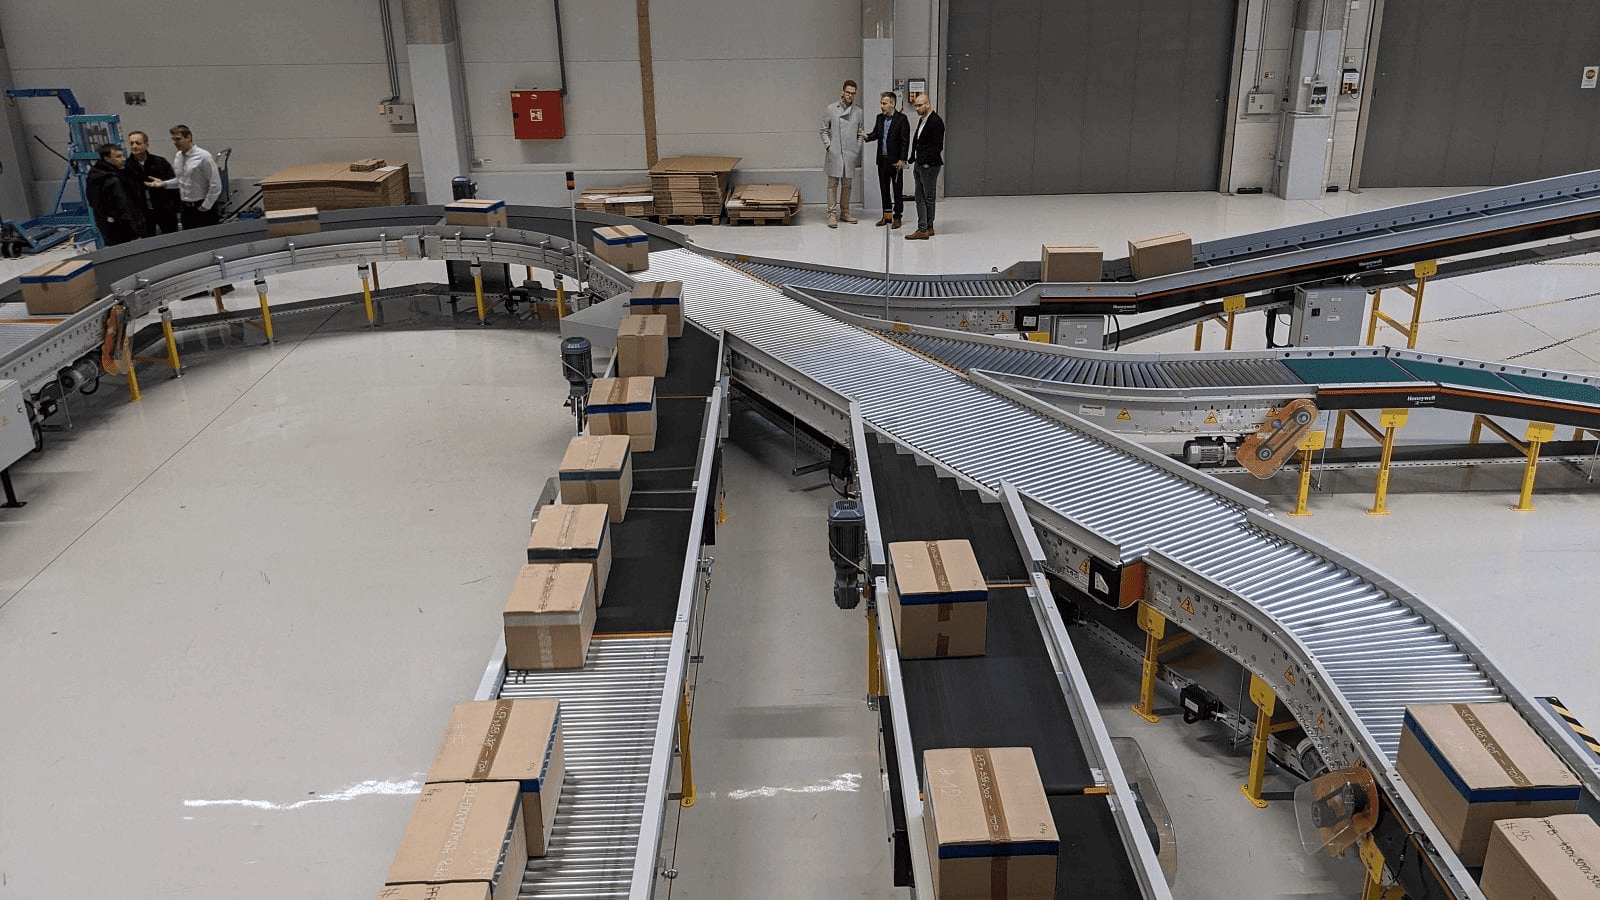
\includegraphics[width=1\linewidth]{images/BrnenskaHoneywellHala.png}
	\caption{Ukázka Brněnské haly pro testování dopravníků společnosti Honeywell \cite{HoneywellHala}}
	\label{fig:BrnenskaHoneywellHala}
\end{figure}

Způsob, jakým byl systém prvně otestován je skrz konfiguraci ovládacího panelu frekvenčního měniče podle instrukcí specifikovaných na stránce "/setup" dostupné uvnitř mobilní aplikace. Nejdříve byla rozpojena výkonová část frekvenčního měniče a poté byl nastavený dle návodu. Po dokončení softwarové konfigurace byla deska připojena na digitální vstupy do ovládacího panelu frekvenčního měniče včetně stejnosměrného $24V$ napájení z výstupního napájecího portu ovládacího panelu.

Po otestování správnosti zapojení a konfigurace pomocí lokálního zapojení byla provedena zkouška s vypnutou výkonovou částí frekvenčního měniče a následně i se zapnutou výkonovou částí frekvenčního měniče, kde se dopravník začal pohybovat, jak bylo předpokládáno. Při uvádění dopravníku do provozu se zapnutou výkonovou částí je potřebné zajistit, aby v systému nebyla načtená hodnota aproximace rychlosti dopravníku jiná než 0. Zanedbání tohoto kroku vede k tomu, že bude systém ukazovat v mobilní aplikaci i na LCD displeji posunutou hodnotu rychlosti.

\section{Ověření lokálního ovládání}
% \purpose{Tady bych se chtěl zaměřit na to, jestli je možné dopravník ovládat přes tlačítka rovnou umístěná na desce.}

Funkčnost lokálního ovládání byla ověřena tím způsobem, že se nejdříve otestovalo, že je možné ovládat dopravník s vypnutou deskou a poté se deska připojila a znovu se testovalo jestli je možné dopravník ovládat s připojenou deskou, která je nastavená na lokální režim ovládání.

Při připojení systému na dopravník bez připojení napájecího kabelu bylo vidět, že LCD displej nefunguje a v mobilní aplikaci není dostupná žádná IP adresa. Dopravník bylo stále možné ovládat, jelikož je deska plošných spojů provedena tím způsobem, že když není napájena, je ovládána lokálně.

Při připojení systému na dopravník s připojením napájecího kabelu se ihned spustil LCD displej a bylo vidět, že se vývojová deska snaží připojit na hotspot. Po připojení bylo možné vidět IP adresu vývojové desky na displeji i v mobilní aplikaci. Při nastavení přepínače na polohu ve kterém je deska lokálně ovládaná bylo stále možné ovládat dopravník pomocí tlačítek na schránce. Potvrdilo se tedy, že v tomto módu ovládání deska neposílá žádné napětí na sepnutí MOSFET transistorů co spínají relé a tak systém stále funguje plně analogově. Při tomto módu zapojení je ale dostupná informace o rychlosti dopravníku jak na LCD displeji tak i v mobilní aplikaci.

\section{Ověření mobilní aplikace}
%\purpose{Tady jenom potvrdím že mobilní aplikace opravdu funguje}

Po úspěšném otestování analogového ovládání desky bylo přistoupeno k testování mobilní aplikace. Mobilní aplikace se už částečně otestovala při předchozím testu, kdy bylo vidět, že pokud je vývojová deska přidaná se správnou IP adresou do aplikace, lze vidět rychlost a způsob ovládání dopravníku i pokud systém není přepnutý do dálkového ovládání.

Pro další testování byl systém přepnutý do stavu dálkového ovládání pomocí přepínače který je umístěný na schránce systému. Při přepnutí do stavu dálkového ovládání dopravník ihned začal zpomalovat, protože bylo přivedené napětí na MOSFET tranzistor, který ovládá relé pro přepínání mezi typy ovládání - rozpojil se tedy obvod, který přiváděl vysokou digitální hodnotu na ON/OFF vstup ovládacího panelu. Následně bylo potvrzeno, že dopravník lze ovládat pomocí mobilní aplikace, která úspěšně posílala GET požadavky na WebServer a tak bylo vidět že vývojová deska přepíná relé, které na desce plošných spojů spíná digitální vstupy ovládacího panelu.

Při přepnutí do dálkového stavu ovládání bylo také v mobilní aplikaci vidět, že se typ ovládání změnil na variantu "Remote".

\section{Spolehlivost dálkové komunikace}
%\purpose{Potvrdit že jsem schopný odejít na několik desítek metrů bez toho abych ztratil signál}

Při zapojení systému s dálkovým ovládáním bylo možné otestovat zároveň i vzdálenost komunikace, které je možné se systémem dosáhnout. Pro otestování dosažitelné vzdálenosti bylo zvoleno jít směrem pryč od druhé spuštěné dopravníkové linky, aby bylo méně pravděpodobné, že se WiFi signál zaruší. V rámci testování byl také celý systém umístěn tak, aby byla zajištěna přímá viditelnost na anténu vycházející ze schránky. Použité mobilní zařízení bylo během testování Nothing Phone. Tímto způsobem byl dosažen dosah WiFi komunikace kolem 35 metrů.

Tento dosah není tak velký, jak bylo předpokládáno, jelikož se předpokládal WiFi dosah až 90 metrů. Dosah systému je menší, jelikož je omezený mobilním zařízením – dosah hotspotů není u běžných Android zařízení parametr, který by se výrobci snažili optimalizovat na maximální hodnotu. Tento dosah je ale pro systém stále přijatelný. Dálkové ovládání je v systému navrženo například pro případy, kdy budou mechanické zkoušky prováděny na dopravnících nainstalovaných pod stropem skladové haly. V těchto případech se výška dopravníků může pohybovat kolem 10 metrů, a tak by měl být dosah 35 metrů dostatečný i pro tyto případy.

Do maximální vzdálenosti nebyly zaznamenány žádné problémy s komunikací. Vývojová deska reagovala okamžitě. Tohle se dalo předpokládat, vzhledem k tomu, že vývojová deska odpovídá na WebServerové požadavky velmi často a jinak není zatížená dlouhými výpočty, které by výrazně zvyšovaly dobu prodlení mezi požadavkem a zpracováním.

\section{Ověření zapojení více desek}
%\purpose{Tady bych se rád zaměřil na nějaké testy, při kterých zkouším, jestli je opravdu možné ovládat víc desek zároveň.}

V rámci tohoto testu byly nakonfigurovány a zapojeny dvě desky dle standardního postupu s tím, že každá deska byla zapojena k samostatnému dopravníku. Dopravníky byly zvoleny tak, aby od sebe byly frekvenční měniče vzdálené v rámci několika metrů a aby bylo možné z jednoho místa vidět antény obou schránek. Obě schránky byly pomocí přepínačů nastaveny na dálkový režim ovládání a IP adresy obou WebServerů byly přidané do mobilní aplikace.

Následně bylo nejdříve s vypnutou výkonovou částí frekvenčního měniče potvrzeno, že aplikace posílá správné GET požadavky na správné WebServery a tak je možné tímto způsobem ovládat oba dopravníky z jedné mobilní aplikace. Toto bylo potvrzeno ještě jednou se zapnutou výkonovou částí frekvenčního měniče s tím, že byly na dopravníky položeny testovací balíky, aby bylo možné vidět, kdy se dopravníky pohybují.

I v případě zapojení více desek komunikovaly WebServery promptně a bez jakýchkoli problémů s komunikací.

\section{Posouzení z hlediska bezpečnosti}\label{sec:PosouzeniZHlediskaBezpecnosti}
%\purpose{Tady bude nějaký moje zamyšlení nad bezpečností téhle desky. }

Navržený systém už ze své podstaty umožňuje dálkové ovládání dopravníkových linek, a to i na delší časové úseky – například při zahořovacích testech, kdy se ověřuje, že je dopravník schopný nepřetržitého provozu. Takovýto způsob ovládání může představovat inherentní riziko v případě ztráty komunikačního spojení mezi mobilní aplikací a vývojovou deskou v kritickém okamžiku, kdy by operátor nemohl dopravník bezprostředně zastavit.

Z tohoto důvodu byla zvažována implementace mechanismu periodické kontroly aktivního spojení (například periodický „ping“ dotaz), který by inicioval zastavení dopravníku, pokud by vývojová deska tento požadavek neobdržela ve stanoveném intervalu. Od implementace takového mechanismu však bylo upuštěno, jelikož by příliš negativně ovlivňoval používání aplikace uživateli. Během provádění těchto dynamických zkoušek uživatelé hledají chyby instalace dopravníkového systému a tyto chyby se běžně zapisují do dokumentace v jiných aplikacích. Dá se tedy předpokládat, že aplikace běžně nebude na mobilním zařízení stále aktivní.

Toto rozhodnutí je podpořeno tím, že navržený systém se spoléhá na již existující bezpečnostní prvky instalované na samotných dopravníkových linkách a přebírá je. Dopravníkové linky mají hned po instalaci standardní bezpečnostní prvky, jako jsou tlačítko nouzového zastavení (E-STOP) a bezpečnostní lanka po celé délce dopravníku.

V kontextu bezpečného provozu je rovněž důležité adekvátní proškolení uživatelů systému. Uživatel musí být seznámen s postupy bezpečného používání systému – hlavně s nutností deaktivace výkonové části frekvenčního měniče pomocí příslušného vypínače před jakoukoliv manipulací s ovládacím panelem. Uživatel musí být dále informován o správném postupu konfigurace systému a o způsobu řešení běžných provozních problémů. Tyto informace jsou obsaženy v mobilní aplikaci na stránkách Setup a Help.